\documentclass[12pt,oneside]{book} % [tamanho da letra,imprimir só frente]{tipo do texto}
\usepackage{graphicx} % pacote para inserir gráfico e figuras
\usepackage{subcaption} % pacote para inserir subfiguras
\usepackage{color} % pacote para usar cor no texto
\usepackage{amscd,amsfonts,amssymb,amsmath,amsthm} % pacotes para o ambiente matemático
\usepackage[utf8]{inputenc} % pacote para permitir o uso do pacote fontec
\usepackage[T1]{fontenc} % pacote para usar a acentuação do teclado
\usepackage[brazil]{babel} % pacote para traduzir chapter/section/contents/... do inglês para o português
\usepackage[all]{xy} % pacote para criar diagramas
\usepackage{enumerate} % pacote para usar itens enumerados
\usepackage[a4paper]{geometry} % pacote para redefinir as dimensões do corpo do texto em um papel a4
\usepackage{fancyhdr} % pacote para personalizar cabeçalho e rodapé
\usepackage{tabularx} % pacote para personalizar o tamanho das tabelas
\usepackage{makeidx} % pacote para criar o índice remissivo

\geometry{textwidth=160mm,textheight=247mm,top=30mm,bottom=20mm,left=30mm,right=20mm,headsep=10mm,footskip=10mm} % {largura do texto,altura do texto,margem superior,margem inferior,margem esquerda,margem direita,distância entre cabeçalho e texto,distância entre rodapé e texto}
% A conta que deve ser feita no comando geometry é a seguinte: papel a4 tem dimensões 210mm x 297mm. Então 210=left + textwidth + right e 297=top + textheight + bottom

\pagestyle{fancy} % comando para configurar cabeçalho e rodapé
\fancyhead[LO]{\leftmark}
\fancyhead[RO]{\thepage}
\fancyfoot[C]{\empty}

\makeindex % comando para começar a montar o índice remissivo





\begin{document}

    \fontfamily{ptm}\selectfont % comando para alterar a fonte usada na digitação de tudo que aparecer daqui pra frente.
    % ptm - Times New Roman

    % ---------------------------------------------------------------------------------------------------
    % ---------------------------------------------------------------------------------------------------
    % --------------------------------------------------------------------------------------------   CAPA
    % ---------------------------------------------------------------------------------------------------
    % ---------------------------------------------------------------------------------------------------





    \begin{titlepage}
        \begin{center}
            \textbf{NOME DA UNIVERSIDADE}
        \end{center}

        \vspace{-0.8cm}

        \begin{center}  
            \scriptsize{NOME DO INSTITUTO}
        \end{center}

        \vspace{-0.8cm}

        \begin{center}
            \scriptsize{PROGRAMA DE PÓS-GRADUAÇÃO EM ???}
        \end{center}

        \vspace{3cm}

        \begin{center}
            \small{Nome do Autor}
        \end{center}

        \vspace{3cm}

        \begin{center}
            \Large{\textbf{Título da Tese}} % caso o título seja grande e ocupe mais de uma linha, talvez será necessário alterar o vspace abaixo, entre o título e o nome da cidade
        \end{center}

        \vspace{12cm}

        \begin{center}
            Cidade - Sigla do Estado
        \end{center}

        \vspace{-0.8cm}
        
        \begin{center}
            Ano
        \end{center}
    \end{titlepage}





    % ---------------------------------------------------------------------------------------------------
    % ---------------------------------------------------------------------------------------------------
    % ----------------------------------------------------------------------------------   FOLHA DE ROSTO
    % ---------------------------------------------------------------------------------------------------
    % ---------------------------------------------------------------------------------------------------





    \newpage
    \thispagestyle{empty} % comando para não aparecer o número da página, mas não interfere na numeração do texto

    \begin{center}
        \small{Nome do Autor}
    \end{center}

    \vspace{3cm}

    \begin{center}
        \Large{\textbf{Título da Tese}} % caso o título seja grande e ocupe mais de uma linha, talvez será necessário alterar o vspace abaixo, entre o título e o nome da cidade. NÃO alterar o vspace entre o título e o comando minipage
    \end{center}

    \vspace{2cm}

    \begin{flushright}
        \begin{minipage}{0.5\textwidth}
            Tese apresentada ao Programa de Pós-Graduação em ?? da Nome da Universidade como parte dos requisitos necessários para a obtenção do título de Doutor em ??
        \end{minipage}
    \end{flushright}

    \vspace{13cm}

    \begin{center}
        Cidade - Sigla do Estado
    \end{center}

    \vspace{-0.8cm}

    \begin{center}
        Ano
    \end{center}





    % ---------------------------------------------------------------------------------------------------
    % ---------------------------------------------------------------------------------------------------
    % ------------------------------------------------------------------------------   FOLHA DE APROVAÇÃO
    % ---------------------------------------------------------------------------------------------------
    % ---------------------------------------------------------------------------------------------------





    \chapter*{Folha de Aprovação}
    \thispagestyle{empty}

    APÓS O PDF ESTAR FINALIZADO, ESTA FOLHA DEVE SER REMOVIDA PARA COLOCAR A FOLHA DE APROVAÇÃO

    esta folha só foi colocada aqui pois deve ser contada na numeração do trabalho

    \vspace{2cm}

    ATENÇÃO: na versão final do pdf, a ficha catalográfica dada pela biblioteca deve estar numa folha a parte e colocada entre a folha de rosto e a folha de aprovação. Já na impressão, TODO o texto deve ser impresso no modo frente, EXCETO pela ficha, que deve ser impressa no verso da folha de rosto!!!





    % ---------------------------------------------------------------------------------------------------
    % ---------------------------------------------------------------------------------------------------
    % -------------------------------------------------------------------------------------   DEDICATÓRIA
    % ---------------------------------------------------------------------------------------------------
    % ---------------------------------------------------------------------------------------------------





    % A DEDICATÓRIA, OS AGRADECIMENTOS E O EPÍGRAFE NÃO SÃO OBRIGRATÓRIOS. CASO NÃO QUEIRA, SÓ DELETAR


    \newpage
    \thispagestyle{empty}

    % a dedicatótio deve ser curta. Caso tenha mais de duas linhas, talvez será necessário alterar o vspace abaixo
    \begin{flushright}
        \begin{minipage}{5cm}
            \begin{flushright}
                \vspace{23cm}\textit{Este espaço é separado para dedicatória.}
            \end{flushright}
        \end{minipage}
    \end{flushright}





    % ---------------------------------------------------------------------------------------------------
    % ---------------------------------------------------------------------------------------------------
    % ----------------------------------------------------------------------------------   AGRADECIMENTOS
    % ---------------------------------------------------------------------------------------------------
    % ---------------------------------------------------------------------------------------------------





    \chapter*{Agradecimentos}
    \thispagestyle{empty}
    % caso os agradecimentos ocupem mais de uma página, NÃO ESQUECER de colocar o comando thispagestyle{empty} nas outras páginas





    % ---------------------------------------------------------------------------------------------------
    % ---------------------------------------------------------------------------------------------------
    % ----------------------------------------------------------------------------------------   EPÍGRAFE
    % ---------------------------------------------------------------------------------------------------
    % ---------------------------------------------------------------------------------------------------





    \newpage
    \thispagestyle{empty}

    % a dedicatótio deve ser curta. Dependendo do número de linhas, será necessário alterar o vspace abaixo. 
    \begin{flushright}
        \begin{minipage}{5cm}
            \begin{flushright}
                \vspace{23cm}\textit{Este espaço é separado para colocar algum texto/citação/mensagem.}
                \vspace{0.2cm}Autor
            \end{flushright}
        \end{minipage}
    \end{flushright}





    % ---------------------------------------------------------------------------------------------------
    % ---------------------------------------------------------------------------------------------------
    % ------------------------------------------------------------------------------------------   RESUMO
    % ---------------------------------------------------------------------------------------------------
    % ---------------------------------------------------------------------------------------------------





    \chapter*{Resumo}
    \thispagestyle{empty}

    Este texto deve ser o resumo do trabalho, sucinto e direto. Não deve haver margem para iniciar o parágrafo. O resumo deve conter no máximo cinco palavras-chaves.

    \

    \noindent Palavras-chaves: palavra 1, palavra 2, palavra 3, palavra 4, palavra 5.
    % o comando noindent é para que não exista margem ao iniciar o parágrafo





    % ---------------------------------------------------------------------------------------------------
    % ---------------------------------------------------------------------------------------------------
    % ----------------------------------------------------------------------------------------   ABSTRACT
    % ---------------------------------------------------------------------------------------------------
    % ---------------------------------------------------------------------------------------------------





    \chapter*{Abstract}
    \thispagestyle{empty}

    This text should be the summary of the work in English, succinct and direct. There should be no margin to start the paragraph. The abstract must contain a maximum of five keywords.

    \

    \noindent Keywords: word 1, word 2, word 3, word 4, word 5.





    % ---------------------------------------------------------------------------------------------------
    % ---------------------------------------------------------------------------------------------------
    % ---------------------------------------------------   SUMÁRIO + LISTA DE FIGURAS + LISTA DE TABELAS
    % ---------------------------------------------------------------------------------------------------
    % ---------------------------------------------------------------------------------------------------





    \tableofcontents % comando para criar o sumário
    \thispagestyle{empty}

    \listoffigures % lista de figuras (caso não for usar, delete ou coloque o símbolo de porcentagem no início da linha)
    \thispagestyle{empty}

    \listoftables % lista de tabelas (caso não for usar, delete ou coloque o símbolo de porcentagem no início da linha)
    \thispagestyle{empty}





    % ---------------------------------------------------------------------------------------------------
    % ---------------------------------------------------------------------------------------------------
    % -------------------------------------------------------------------------------   LISTA DE NOTAÇÕES
    % ---------------------------------------------------------------------------------------------------
    % ---------------------------------------------------------------------------------------------------





    \chapter*{Lista de Notações}
    \thispagestyle{empty}
    % caso a lista de notações ocupe mais de uma página, NÃO ESQUECER de colocar o comando thispagestyle{empty} nas outras páginas





    % ---------------------------------------------------------------------------------------------------
    % ---------------------------------------------------------------------------------------------------
    % --------------------------------------------------------------------------------------   INTRODUÇÃO
    % ---------------------------------------------------------------------------------------------------
    % ---------------------------------------------------------------------------------------------------





    \chapter{Introdução}
    \thispagestyle{empty}
    % nenhuma página antes da introdução deve conter o número da página, mas a numeração deve ser iniciada a partir da folha de rosto, exceto a página da ficha catalográfica, que deve ser impressa no verso da folha de rosto. Os comandos feitos até agora já obedecem essa regra da numeração
    % NENHUM CAPÍTULO DEVE CONTER A NUMERAÇÃO NA SUA PRIMEIRA PÁGINA. SEMPRE QUE ADICIONAR OUTROS CAPÍTULOS, NÃO ESQUECER DE COLOCAR O COMANDO THISPAGESTYLE{EMPTY} APÓS O COMANDO CHAPTER





    % ---------------------------------------------------------------------------------------------------
    % ---------------------------------------------------------------------------------------------------
    % ---------------------------------------------------------------------------------   DESENVOLVIMENTO
    % ---------------------------------------------------------------------------------------------------
    % ---------------------------------------------------------------------------------------------------





    \chapter{Desenvolvimento}
    \thispagestyle{empty}

    \

    \par Teorema do Posto \index{Teorema!do Posto}

    \par Vejamos um exemplo de tabela e como inserir na lista de tabelas: \vspace{1.5cm}

    \begin{table}[h] % comando para poder citar a tabela. Ainda, [h] é para que a tabela apareça onde você colocou, e não onde a compilação mandar. Experimente tirar o [h] e veja no que dá
        \begin{center}
            \begin{tabular}{|l|c||lr} % comando para se criar tabela
                \hline
                \multicolumn{4}{|c|}{Calendário} \\ \hline \hline
                jan & fev & mar & abr \\ \hline
                mai & & jun & jul \\ \cline{1-1} \cline{3-4}
                ago & set & & out \\
                nov & & & dez
            \end{tabular}
        \end{center}
        \caption{exemplo de tabela}
    \end{table}

    \vspace{1.5cm}

    \par Por outro lado, é possível personalizar o tamanho da tabela, como no seguinte exemplo:

    \begin{table}[h]
        \begin{center}
            \begin{tabularx}{10cm}{|X|c||Xr} % as colunas especificadas por X terão a mesma largura
                \hline 
                \multicolumn{4}{|c|}{Calendário} \\ \hline \hline
                jan & fev & mar & abr \\ \hline
                mai & & jun & jul \\ \cline{1-1} \cline{3-4}
                ago & set & & out \\
                nov & & & dez
            \end{tabularx}
        \end{center}
        \caption{exemplo de tabela com tamanho personalizado}
    \end{table}

    \section{Teste}

    \

    \par Axioma das paralelas \index{Axioma das paralelas}

    \par Agora, vejamos um exemplo de figura e como inserir na lista de figuras: % o arquivo da figura deve estar na mesma pasta do arquivo tex

    \begin{figure}[h] % justificativa do [h] é a mesma para o comando table
        \begin{center}
            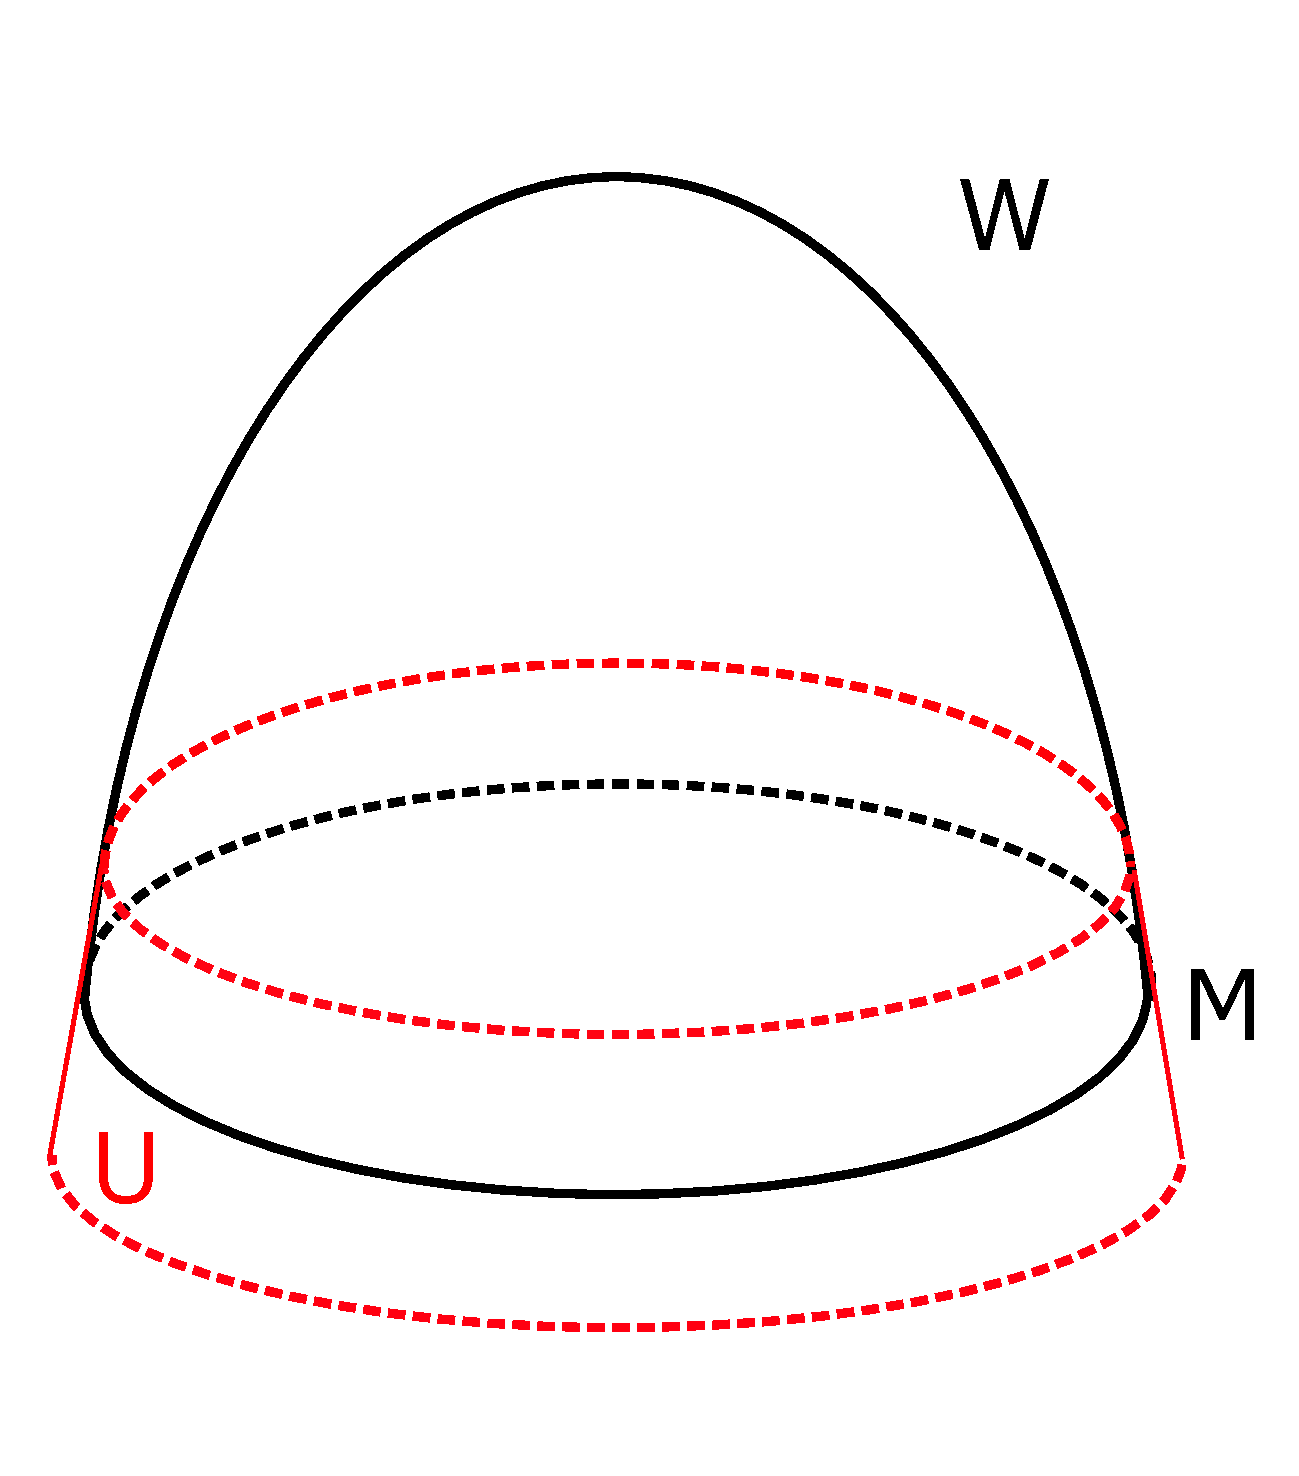
\includegraphics[scale=0.2]{varied_c_bordo.pdf}
        \end{center}
        \caption{exemplo de figura}
    \end{figure}

    \subsection{Subteste}

    \

    \par Teorema do isomorfismo \index{Teorema!do isomorfismo}\footnote{Este Teorema pode ser encontrado em \cite{exemplo 1}}

    \par Por fim, vejamos um exemplo de subfigura e como inserir na lista de figuras: \vspace{1.5cm}

    \begin{figure}[h]
        \begin{center}
            \begin{subfigure}[b]{0.45\textwidth} % largura da subfigura pode ser ajustada conforme necessário
                \centering
                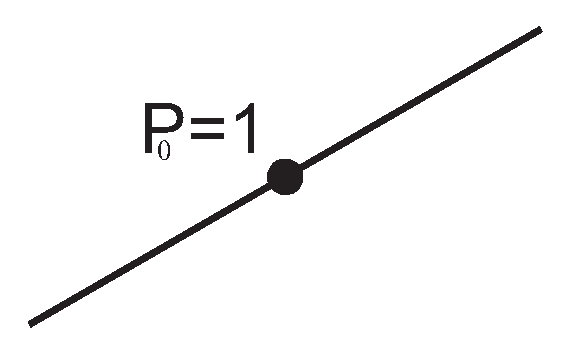
\includegraphics[scale=0.25]{gr1.pdf}
                \caption{0-simplexo}
            \end{subfigure}
            \hspace{0.5cm}
            \begin{subfigure}[b]{0.45\textwidth}
                \centering
                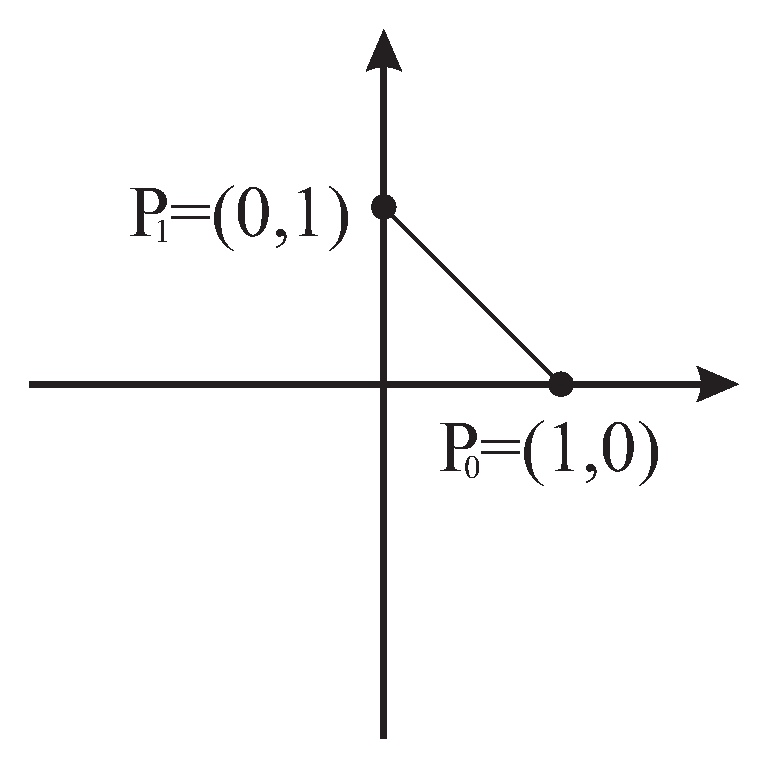
\includegraphics[scale=0.25]{gr2.pdf}
                \caption{1-simplexo}
            \end{subfigure}
        \end{center}
        \caption{Exemplo de subfiguras}
    \end{figure}





    % ---------------------------------------------------------------------------------------------------
    % ---------------------------------------------------------------------------------------------------
    % ---------------------------------------------------------------------------------------   CONCLUSÃO
    % ---------------------------------------------------------------------------------------------------
    % ---------------------------------------------------------------------------------------------------





    \chapter{Conclusão}
    \thispagestyle{empty}





    % ---------------------------------------------------------------------------------------------------
    % ---------------------------------------------------------------------------------------------------
    % ----------------------------------------------------------------------   Referências Bibliográficas
    % ---------------------------------------------------------------------------------------------------
    % ---------------------------------------------------------------------------------------------------





    \begin{thebibliography}{99}
    \thispagestyle{empty}
    \addcontentsline{toc}{chapter}{Referências Bibliográficas} % comando para se adicionar no tableofcontents (toc) como capítulo e com o título referente

    \bibitem{exemplo 1} SOBRENOME, N. {\bf Título.} Nome da revista, v.? (volume), p.?-? (páginas), ano. % exemplo de como referenciar artigo
    
    \bibitem{exemplo 2} SOBRENOME, N. {\bf Título.} Cidade: Editora, ano. % exemplo de como referenciar livro

    \end{thebibliography}





    % ---------------------------------------------------------------------------------------------------
    % ---------------------------------------------------------------------------------------------------
    % ---------------------------------------------------------------------------------------   APÊNDICES
    % ---------------------------------------------------------------------------------------------------
    % ---------------------------------------------------------------------------------------------------





    \appendix % comando para que os capítulos seguintes aparecem como Apêndices

    \chapter{Anexo}
    \thispagestyle{empty}





    % ---------------------------------------------------------------------------------------------------
    % ---------------------------------------------------------------------------------------------------
    % --------------------------------------------------------------------------------   Índice Remissivo
    % ---------------------------------------------------------------------------------------------------
    % ---------------------------------------------------------------------------------------------------





    \newpage

    \addcontentsline{toc}{chapter}{Índice Remissivo}
    \thispagestyle{empty}
    \printindex % comando para adicionar o índice remissivo

    % sempre que for adicionar uma nova palavra no índice remissivo, fazer a seguinte sequência de compilação antes de ver o pdf: 
    %pdflatex + makeindex + pdflatex

\end{document}